\section{Model2DRigid\-Dyncar  Class Reference}
\label{classModel2DRigidDyncar}\index{Model2DRigidDyncar@{Model2DRigid\-Dyncar}}
A 5DOF dynamical model of a rigid car. This model uses a linear tire model, which is far from reality. The model was donated by Jim Bernard. 


{\tt \#include $<$model2d.h$>$}

Inheritance diagram for Model2DRigid\-Dyncar::\begin{figure}[H]
\begin{center}
\leavevmode
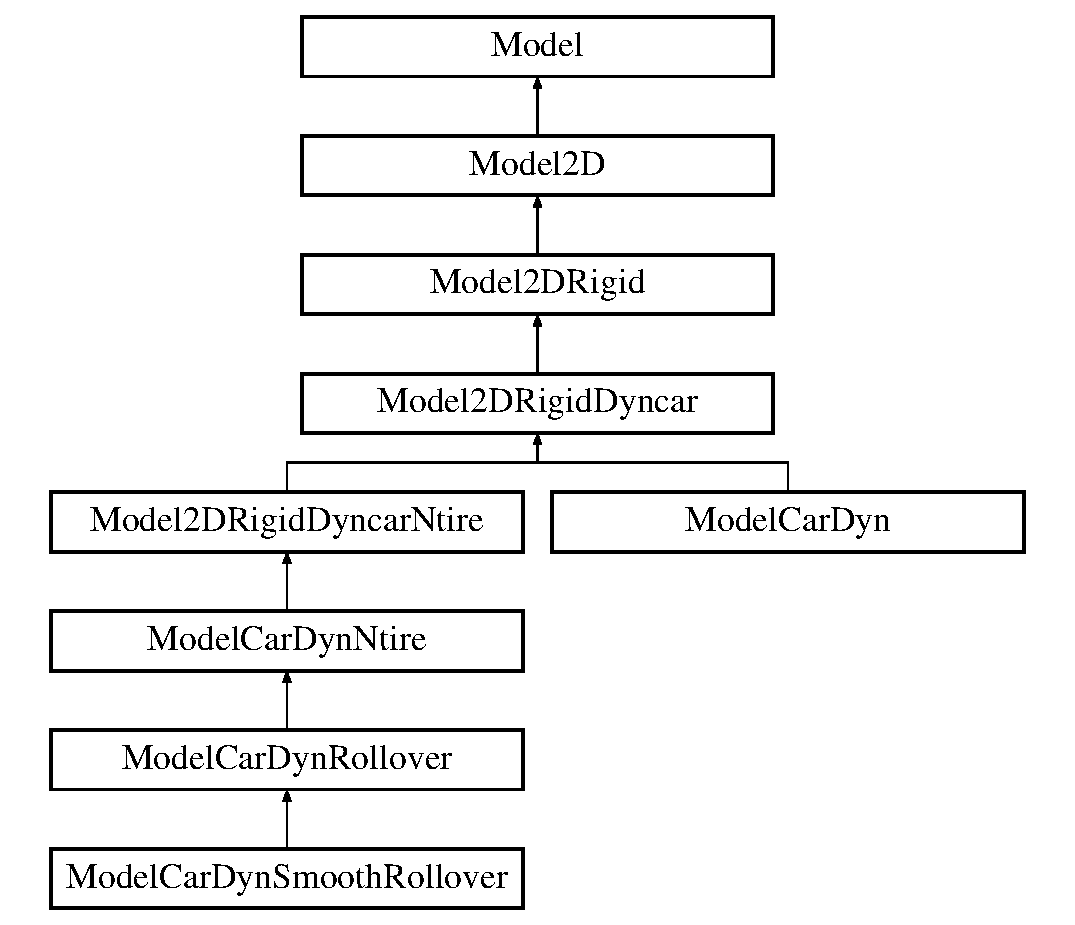
\includegraphics[height=8cm]{classModel2DRigidDyncar}
\end{center}
\end{figure}
\subsection*{Public Methods}
\begin{CompactItemize}
\item 
{\bf Model2DRigid\-Dyncar} (string path)
\item 
virtual {\bf $\sim$Model2DRigid\-Dyncar} ()
\item 
{\bf MSLVector} {\bf Integrate} (const {\bf MSLVector} \&{\bf x}, const {\bf MSLVector} \&u, const double \&h)
\begin{CompactList}\small\item\em Perform integration from state x, using input u, over time step h.\item\end{CompactList}\item 
virtual {\bf MSLVector} {\bf State\-To\-Configuration} (const {\bf MSLVector} \&{\bf x})
\begin{CompactList}\small\item\em A method that converts a {\bf Model} {\rm (p.\,\pageref{classModel})} state in to a {\bf Geom} {\rm (p.\,\pageref{classGeom})} configuration.\item\end{CompactList}\item 
virtual {\bf MSLVector} {\bf State\-Transition\-Equation} (const {\bf MSLVector} \&{\bf x}, const {\bf MSLVector} \&u)
\begin{CompactList}\small\item\em The state transition equation, or equations of motion, xdot=f(x,u).\item\end{CompactList}\item 
virtual double {\bf Metric} (const {\bf MSLVector} \&x1, const {\bf MSLVector} \&x2)
\begin{CompactList}\small\item\em A distance metric, which is Euclidean in the base class.\item\end{CompactList}\item 
virtual {\bf MSLVector} {\bf Linear\-Interpolate} (const {\bf MSLVector} \&x1, const {\bf MSLVector} \&x2, const double \&a)
\begin{CompactList}\small\item\em Linearly interpolate two state while respecting topology.\item\end{CompactList}\item 
virtual {\bf MSLVector} {\bf State\-Difference} (const {\bf MSLVector} \&x1, const {\bf MSLVector} \&x2)
\begin{CompactList}\small\item\em Compute a {\bf MSLVector} {\rm (p.\,\pageref{classMSLVector})} based on x2-x1. In R$^\wedge$n, the states are simply subtracted to make the {\bf MSLVector} {\rm (p.\,\pageref{classMSLVector})}. This method exists to make things work correctly for other state-space topologies.\item\end{CompactList}\end{CompactItemize}
\subsection*{Public Attributes}
\begin{CompactItemize}
\item 
double {\bf Mass}
\begin{CompactList}\small\item\em Mass in slugs (yuck! American customary units...).\item\end{CompactList}\item 
double {\bf CAF}
\begin{CompactList}\small\item\em Front cornering stiffness.\item\end{CompactList}\item 
double {\bf CAR}
\begin{CompactList}\small\item\em Rear cornering stiffness.\item\end{CompactList}\item 
double {\bf Adist}
\begin{CompactList}\small\item\em Mass center to front tires - feet.\item\end{CompactList}\item 
double {\bf Bdist}
\begin{CompactList}\small\item\em Mass center to rear tires - feet.\item\end{CompactList}\item 
double {\bf Izz}
\begin{CompactList}\small\item\em Yaw moment of interia - ft slugs$^\wedge$2.\item\end{CompactList}\item 
double {\bf World\-Scale}
\begin{CompactList}\small\item\em Feet per world unit (100x100 world).\item\end{CompactList}\item 
double {\bf Max\-Steering\-Angle}
\begin{CompactList}\small\item\em Maximum steering angle in radians.\item\end{CompactList}\item 
double {\bf Speed}
\begin{CompactList}\small\item\em A forward speed of the car.\item\end{CompactList}\end{CompactItemize}


\subsection{Detailed Description}
A 5DOF dynamical model of a rigid car. This model uses a linear tire model, which is far from reality. The model was donated by Jim Bernard.



\subsection{Constructor \& Destructor Documentation}
\index{Model2DRigidDyncar@{Model2DRigid\-Dyncar}!Model2DRigidDyncar@{Model2DRigidDyncar}}
\index{Model2DRigidDyncar@{Model2DRigidDyncar}!Model2DRigidDyncar@{Model2DRigid\-Dyncar}}
\subsubsection{\setlength{\rightskip}{0pt plus 5cm}Model2DRigid\-Dyncar::Model2DRigid\-Dyncar (string {\em path})}\label{classModel2DRigidDyncar_a0}


\index{Model2DRigidDyncar@{Model2DRigid\-Dyncar}!~Model2DRigidDyncar@{$\sim$Model2DRigidDyncar}}
\index{~Model2DRigidDyncar@{$\sim$Model2DRigidDyncar}!Model2DRigidDyncar@{Model2DRigid\-Dyncar}}
\subsubsection{\setlength{\rightskip}{0pt plus 5cm}virtual Model2DRigid\-Dyncar::$\sim$Model2DRigid\-Dyncar ()\hspace{0.3cm}{\tt  [inline, virtual]}}\label{classModel2DRigidDyncar_a1}




\subsection{Member Function Documentation}
\index{Model2DRigidDyncar@{Model2DRigid\-Dyncar}!Integrate@{Integrate}}
\index{Integrate@{Integrate}!Model2DRigidDyncar@{Model2DRigid\-Dyncar}}
\subsubsection{\setlength{\rightskip}{0pt plus 5cm}{\bf MSLVector} Model2DRigid\-Dyncar::Integrate (const {\bf MSLVector} \& {\em x}, const {\bf MSLVector} \& {\em u}, const double \& {\em h})\hspace{0.3cm}{\tt  [virtual]}}\label{classModel2DRigidDyncar_a2}


Perform integration from state x, using input u, over time step h.



Reimplemented from {\bf Model2DRigid} {\rm (p.\,\pageref{classModel2DRigid_a2})}.

Reimplemented in {\bf Model\-Car\-Dyn\-Rollover} {\rm (p.\,\pageref{classModelCarDynRollover_a5})}.\index{Model2DRigidDyncar@{Model2DRigid\-Dyncar}!LinearInterpolate@{LinearInterpolate}}
\index{LinearInterpolate@{LinearInterpolate}!Model2DRigidDyncar@{Model2DRigid\-Dyncar}}
\subsubsection{\setlength{\rightskip}{0pt plus 5cm}{\bf MSLVector} Model2DRigid\-Dyncar::Linear\-Interpolate (const {\bf MSLVector} \& {\em x1}, const {\bf MSLVector} \& {\em x2}, const double \& {\em a})\hspace{0.3cm}{\tt  [virtual]}}\label{classModel2DRigidDyncar_a6}


Linearly interpolate two state while respecting topology.

If a=0, then x1 is returned; if a=1, then x2 is returned. All intermediate values of \$a $\backslash$in [0,1]\$ yield intermediate states. This method is defined by {\bf Model} {\rm (p.\,\pageref{classModel})}. 

Reimplemented from {\bf Model2DRigid} {\rm (p.\,\pageref{classModel2DRigid_a4})}.

Reimplemented in {\bf Model\-Car\-Dyn\-Smooth\-Rollover} {\rm (p.\,\pageref{classModelCarDynSmoothRollover_a5})}.\index{Model2DRigidDyncar@{Model2DRigid\-Dyncar}!Metric@{Metric}}
\index{Metric@{Metric}!Model2DRigidDyncar@{Model2DRigid\-Dyncar}}
\subsubsection{\setlength{\rightskip}{0pt plus 5cm}double Model2DRigid\-Dyncar::Metric (const {\bf MSLVector} \& {\em x1}, const {\bf MSLVector} \& {\em x2})\hspace{0.3cm}{\tt  [virtual]}}\label{classModel2DRigidDyncar_a5}


A distance metric, which is Euclidean in the base class.



Reimplemented from {\bf Model2DRigid} {\rm (p.\,\pageref{classModel2DRigid_a6})}.

Reimplemented in {\bf Model\-Car\-Dyn} {\rm (p.\,\pageref{classModelCarDyn_a3})}.\index{Model2DRigidDyncar@{Model2DRigid\-Dyncar}!StateDifference@{StateDifference}}
\index{StateDifference@{StateDifference}!Model2DRigidDyncar@{Model2DRigid\-Dyncar}}
\subsubsection{\setlength{\rightskip}{0pt plus 5cm}{\bf MSLVector} Model2DRigid\-Dyncar::State\-Difference (const {\bf MSLVector} \& {\em x1}, const {\bf MSLVector} \& {\em x2})\hspace{0.3cm}{\tt  [virtual]}}\label{classModel2DRigidDyncar_a7}


Compute a {\bf MSLVector} {\rm (p.\,\pageref{classMSLVector})} based on x2-x1. In R$^\wedge$n, the states are simply subtracted to make the {\bf MSLVector} {\rm (p.\,\pageref{classMSLVector})}. This method exists to make things work correctly for other state-space topologies.



Reimplemented from {\bf Model2DRigid} {\rm (p.\,\pageref{classModel2DRigid_a5})}.\index{Model2DRigidDyncar@{Model2DRigid\-Dyncar}!StateToConfiguration@{StateToConfiguration}}
\index{StateToConfiguration@{StateToConfiguration}!Model2DRigidDyncar@{Model2DRigid\-Dyncar}}
\subsubsection{\setlength{\rightskip}{0pt plus 5cm}{\bf MSLVector} Model2DRigid\-Dyncar::State\-To\-Configuration (const {\bf MSLVector} \& {\em x})\hspace{0.3cm}{\tt  [virtual]}}\label{classModel2DRigidDyncar_a3}


A method that converts a {\bf Model} {\rm (p.\,\pageref{classModel})} state in to a {\bf Geom} {\rm (p.\,\pageref{classGeom})} configuration.



Reimplemented from {\bf Model2DRigid} {\rm (p.\,\pageref{classModel2DRigid_a7})}.

Reimplemented in {\bf Model\-Car\-Dyn} {\rm (p.\,\pageref{classModelCarDyn_a2})}.\index{Model2DRigidDyncar@{Model2DRigid\-Dyncar}!StateTransitionEquation@{StateTransitionEquation}}
\index{StateTransitionEquation@{StateTransitionEquation}!Model2DRigidDyncar@{Model2DRigid\-Dyncar}}
\subsubsection{\setlength{\rightskip}{0pt plus 5cm}{\bf MSLVector} Model2DRigid\-Dyncar::State\-Transition\-Equation (const {\bf MSLVector} \& {\em x}, const {\bf MSLVector} \& {\em u})\hspace{0.3cm}{\tt  [virtual]}}\label{classModel2DRigidDyncar_a4}


The state transition equation, or equations of motion, xdot=f(x,u).



Reimplemented from {\bf Model2DRigid} {\rm (p.\,\pageref{classModel2DRigid_a3})}.

Reimplemented in {\bf Model2DRigid\-Dyncar\-Ntire} {\rm (p.\,\pageref{classModel2DRigidDyncarNtire_a2})}.

\subsection{Member Data Documentation}
\index{Model2DRigidDyncar@{Model2DRigid\-Dyncar}!Adist@{Adist}}
\index{Adist@{Adist}!Model2DRigidDyncar@{Model2DRigid\-Dyncar}}
\subsubsection{\setlength{\rightskip}{0pt plus 5cm}double Model2DRigid\-Dyncar::Adist}\label{classModel2DRigidDyncar_m3}


Mass center to front tires - feet.

\index{Model2DRigidDyncar@{Model2DRigid\-Dyncar}!Bdist@{Bdist}}
\index{Bdist@{Bdist}!Model2DRigidDyncar@{Model2DRigid\-Dyncar}}
\subsubsection{\setlength{\rightskip}{0pt plus 5cm}double Model2DRigid\-Dyncar::Bdist}\label{classModel2DRigidDyncar_m4}


Mass center to rear tires - feet.

\index{Model2DRigidDyncar@{Model2DRigid\-Dyncar}!CAF@{CAF}}
\index{CAF@{CAF}!Model2DRigidDyncar@{Model2DRigid\-Dyncar}}
\subsubsection{\setlength{\rightskip}{0pt plus 5cm}double Model2DRigid\-Dyncar::CAF}\label{classModel2DRigidDyncar_m1}


Front cornering stiffness.

\index{Model2DRigidDyncar@{Model2DRigid\-Dyncar}!CAR@{CAR}}
\index{CAR@{CAR}!Model2DRigidDyncar@{Model2DRigid\-Dyncar}}
\subsubsection{\setlength{\rightskip}{0pt plus 5cm}double Model2DRigid\-Dyncar::CAR}\label{classModel2DRigidDyncar_m2}


Rear cornering stiffness.

\index{Model2DRigidDyncar@{Model2DRigid\-Dyncar}!Izz@{Izz}}
\index{Izz@{Izz}!Model2DRigidDyncar@{Model2DRigid\-Dyncar}}
\subsubsection{\setlength{\rightskip}{0pt plus 5cm}double Model2DRigid\-Dyncar::Izz}\label{classModel2DRigidDyncar_m5}


Yaw moment of interia - ft slugs$^\wedge$2.

\index{Model2DRigidDyncar@{Model2DRigid\-Dyncar}!Mass@{Mass}}
\index{Mass@{Mass}!Model2DRigidDyncar@{Model2DRigid\-Dyncar}}
\subsubsection{\setlength{\rightskip}{0pt plus 5cm}double Model2DRigid\-Dyncar::Mass}\label{classModel2DRigidDyncar_m0}


Mass in slugs (yuck! American customary units...).

\index{Model2DRigidDyncar@{Model2DRigid\-Dyncar}!MaxSteeringAngle@{MaxSteeringAngle}}
\index{MaxSteeringAngle@{MaxSteeringAngle}!Model2DRigidDyncar@{Model2DRigid\-Dyncar}}
\subsubsection{\setlength{\rightskip}{0pt plus 5cm}double Model2DRigid\-Dyncar::Max\-Steering\-Angle}\label{classModel2DRigidDyncar_m7}


Maximum steering angle in radians.

\index{Model2DRigidDyncar@{Model2DRigid\-Dyncar}!Speed@{Speed}}
\index{Speed@{Speed}!Model2DRigidDyncar@{Model2DRigid\-Dyncar}}
\subsubsection{\setlength{\rightskip}{0pt plus 5cm}double Model2DRigid\-Dyncar::Speed}\label{classModel2DRigidDyncar_m8}


A forward speed of the car.

\index{Model2DRigidDyncar@{Model2DRigid\-Dyncar}!WorldScale@{WorldScale}}
\index{WorldScale@{WorldScale}!Model2DRigidDyncar@{Model2DRigid\-Dyncar}}
\subsubsection{\setlength{\rightskip}{0pt plus 5cm}double Model2DRigid\-Dyncar::World\-Scale}\label{classModel2DRigidDyncar_m6}


Feet per world unit (100x100 world).



The documentation for this class was generated from the following files:\begin{CompactItemize}
\item 
{\bf model2d.h}\item 
{\bf model2d.C}\end{CompactItemize}
